% Charlotte Geiger - Manuel Lippert - Leonard Schatt
% Physikalisches Praktikum

% Teilaufgabe X

\section{Das elektromagnetische Spektrum}


\begin{figure}[h]
    \centering
    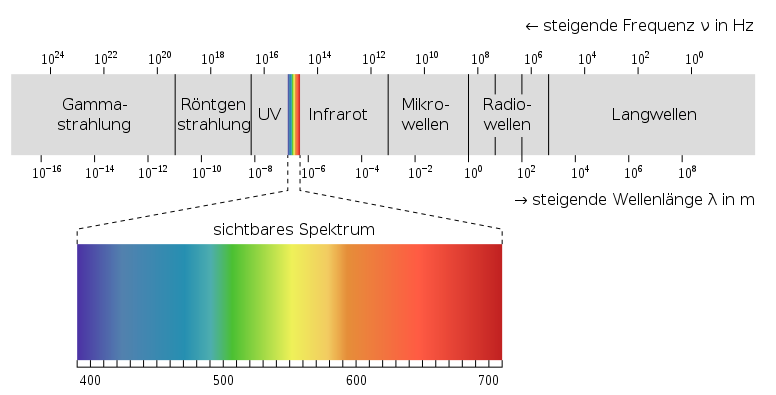
\includegraphics[width=\linewidth]{Bilder/Emspekt.PNG}
    \caption{Das elektromagnetische Spektrum\protect\footnotemark}
    %\label{fig:meine-grafik}
\end{figure}
\footnotetext{\url{https://de.m.wikipedia.org/wiki/Datei:EM-Spektrum.svg}}
\begin{itemize}
    \item Gammastrahlung: Gammastrahlung entsteht bei Radioaktiven zerfällen, wie beispielsweise Selen mit der Nuklidzahl 70. Detektieren kann man die Strahlung mit einer Nebelkammer oder einem Geiger-Müller-Zählrohr.
    \item Röntgenstrahlung: Diese Strahlung wird in der Medizin und in der Industrie viel eingesetzt zur Untersuchung von Materialen. Die Röntgenstrahlungwird dabei in einer Röntgenröhre durch das abbremsen von schnellen Elektronen erzeugt. Man kann die Strahlung durch Fotoplatten nachweisen.
    \item UV: UV-Strahlung entsteht in der Sonne. Sie ist noch hochenergetisch genug um erbgutschädigend zu wirken. Man kann sie mir Fotoplatten oder über den Fotoeffekt nachweisen.
    \item Sichtbares Licht: Dieses wird von der Sonne emmitiert. Nachweisen kann man es mit der Sonne oder einem Fotowiderstand und einem entsprechendem Messgerät.
    \item Infrarot: Infrarotstrahlung entsteht auch in der Sonne. Man kann sie durch thermische Detektoren wie Bolometer nachweisen.
    \item Mikrowellen: Die wohl bekannteste technische Anwendung ist der "Mikrowellenherd". Dort werden die Wellen durch einen Magnetron erzeugt. Nachweisen kann man sie mit einer passenden Antennen und einem Messgerät. Die länge der Antenne muss zur Welle passen.
    \item Radiowellen: Diese könne naturlich entstehen. Dort werden sie duch die Temperatur der Atmosphäre selbst erzeugt. Detektieren kann man die Wellen mit einer passenden Dipolantenne.
    \item Langwellen: Langwellen können von Langwellensendern gesendet werden. Empfangen kann man sie mit einer passenden Dipolantenne.
\end{itemize}